مسائل ۳۰.۱۳ و ۲۰.۱۳ از کتاب \lr{Roth}


%دیاگرام حالت زیر:
%
%\begin{enumerate}
%	\item 
%	مدل میلی است یا مور؟
%	
%	\item 
%	اگر مور است، آن را به میلی و اگر میلی است آن را به مور تبدیل کنید.\\
%	(راهنمایی: باتوجه به تعریف و تفاوت مدل میلی و مور بررسی کنید چطور می‌توانید تبدیل را انجام دهید.)
%\end{enumerate}
%
%\begin{figure}[h]
%	\centering
%	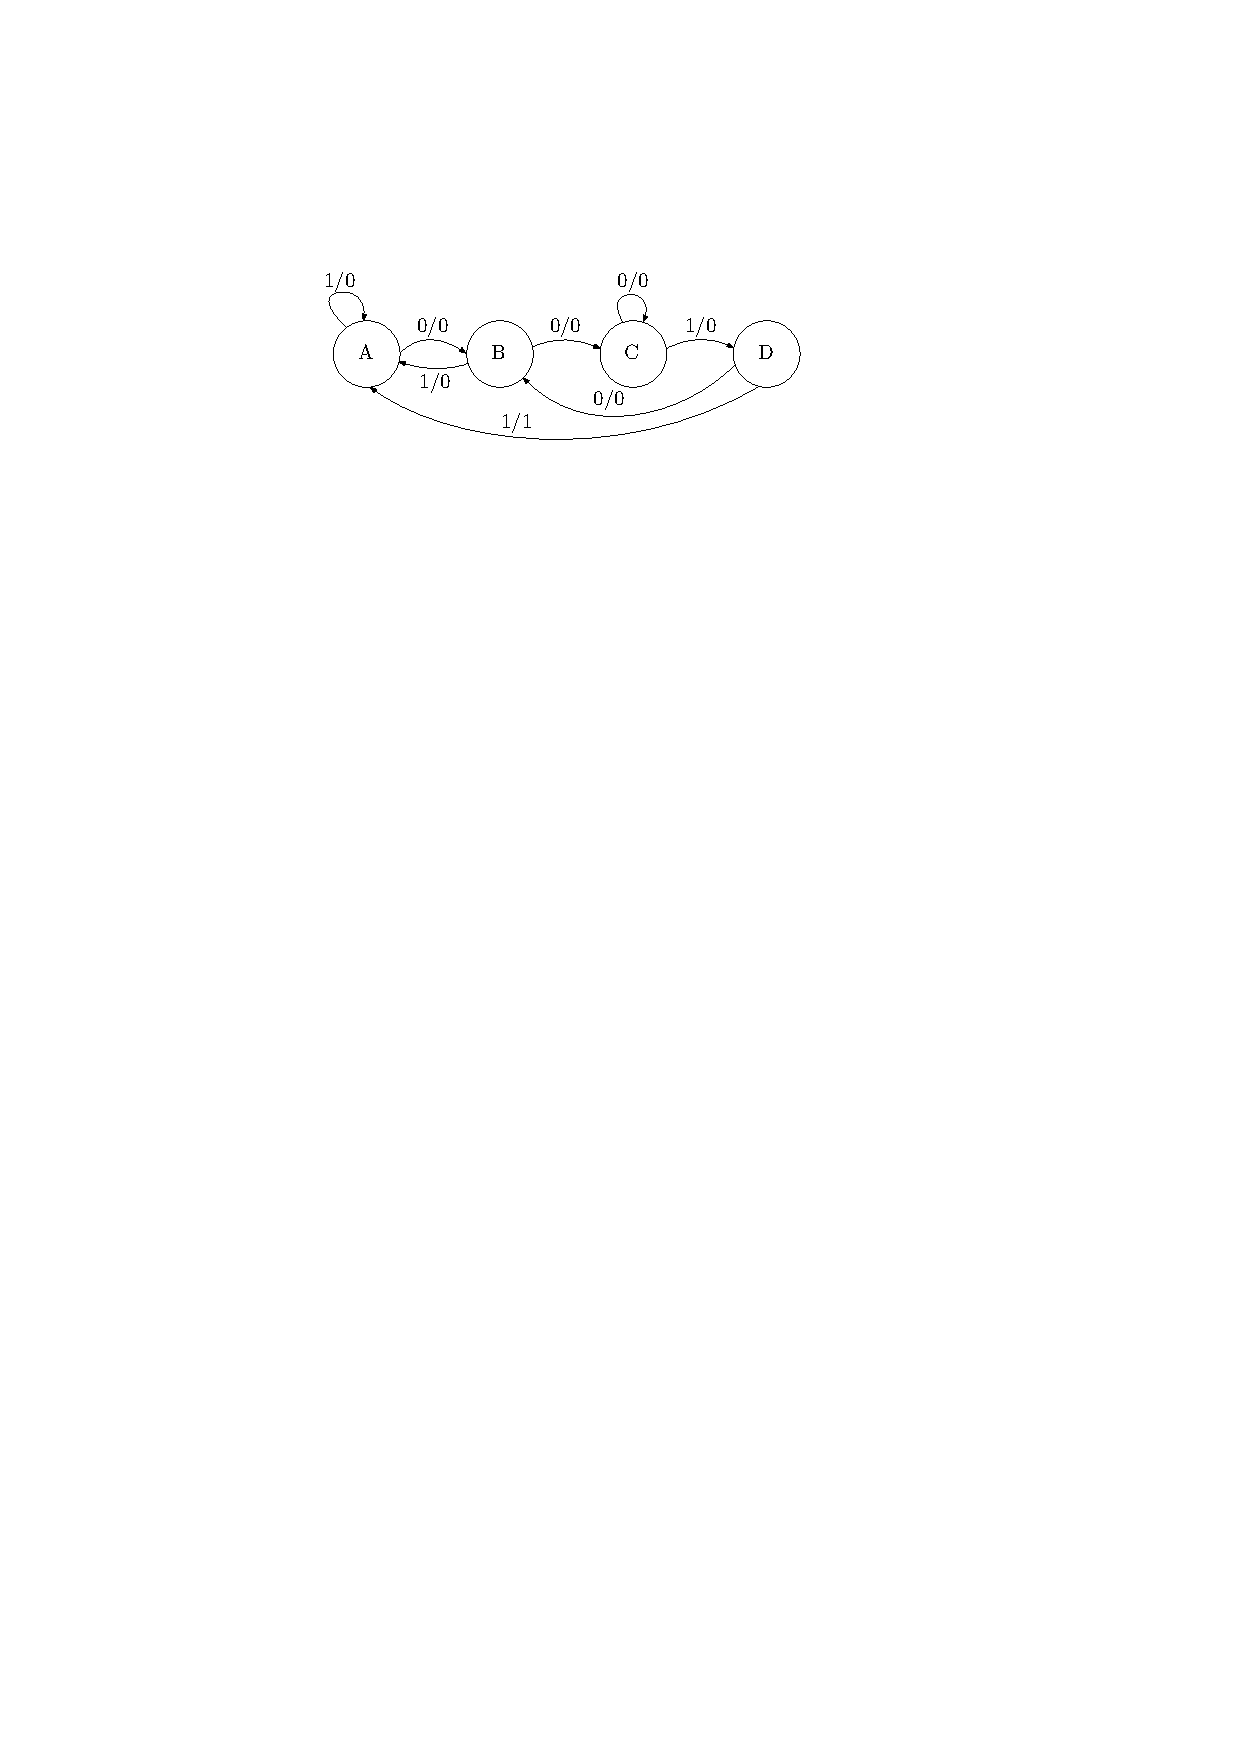
\includegraphics[width=0.6\textwidth]{fig/Q_basic9.pdf}
%	\label{fig:Q_basic_9}
%\end{figure}